\chapter{Introduction}\label{ch:intro}

\section{Motivation}\label{motivation}
\hspace*{0.5cm} Today, after the Covid - 19 pandemic \cite{covid}, information technology is moving at an incredible speed within Kazakhstan and around the world, many online learning platforms are being created where users learn new skills and apply them in practice. Our SkillSwap \cite{skillswap} project aims to unite students into one community where they can exchange skills, ask questions, and answer them, it is a mutually beneficial exchange of skills, and a student can also receive funding for his project if he really innovates, if the investor himself sees it.The platform itself allows you to find other students who are also interested in learning something new, and a paid exchange is also possible, depending on the purpose of the students. The motivation and mission of our project itself come from effective learning, proper planning, and application of new knowledge in practice (depends on the motivation and vision of the students themselves); our platform is the place (together) where students can find and learn something new, answers to questions within the platform, that is, each student can ask a question and answer it and also give a rating to the question, that is, is the question good or not, all students should know how to ask a question to learn this -  nometa.xyz \cite{nometa} encouraging students to correctly use communication skills that will be useful to them in the future. Today there is such a problem that students are afraid to communicate, to make new acquaintances. There is a risk that a student after graduation will not find friends and connections and will grieve about this. In the next chapters, we will consider this problem in more detail.

\newpage
\section{Aims and Objectives}\label{aimsobj}
\justifying
\hspace*{0.5cm} Our project objective is to create a platform for students to mutually benefit from the exchange of skills in order to learn something new and find new connections within the people and university, as well as being able to ask any question on the platform and answer others, and implement a crowdfunding platform \cite{crowdfunding} for devouring any project. Taking this into account, we next identified \nameref{aimsobj}.

\par
\flushleft
\textbf{Aims:}
\begin{itemize}
\justifying
  \item Creating a platform within the university aimed at exchanging skills between students in order to improve their communication skills and technique skills.
  \item Increasing students ability to use the platform to share knowledge and experiences, giving them the opportunity to ask questions, answer them and evaluate their usefulness, similar to popular resources like Stack Overflow \cite{stackoverlow} and headhunter.kz \cite{headhunter} or reddit.com \cite{reddit}.
  \item Support student’s projects on the platform by providing them with tools to finance them and implement their ideas, including using a donation system that allows investors to support promising projects.
\end{itemize}

\textbf{Objectives:}
\begin{itemize}
\justifying
  \item The development of a website (describes in \nameref{back} part) platform and an application \nameref{ios} that makes it possible to register on the platform, which makes it possible to use 100 percent of the platform's functionality and also create their profiles.
  \item The development of a kind of mechanism for the exchange of skills, and this is a chat so that users can communicate, also ask questions and give answers to them, and also rate the question whether it is correctly asked or not.
  \item Creating a crowdfunding \cite{crowdfunding} section for the exhibition of personal projects from students who need financing for future investors.
  \item Creating a simple and proper interface for users to use the application better.
  \item Implement security for users of SHA-256 data encryption and personal chat history information.  
\end{itemize}

\newpage
\section{Problem statement}\label{prblstatm}
\begin{figure}[ht]\label{fig:sstats}
  \centering
  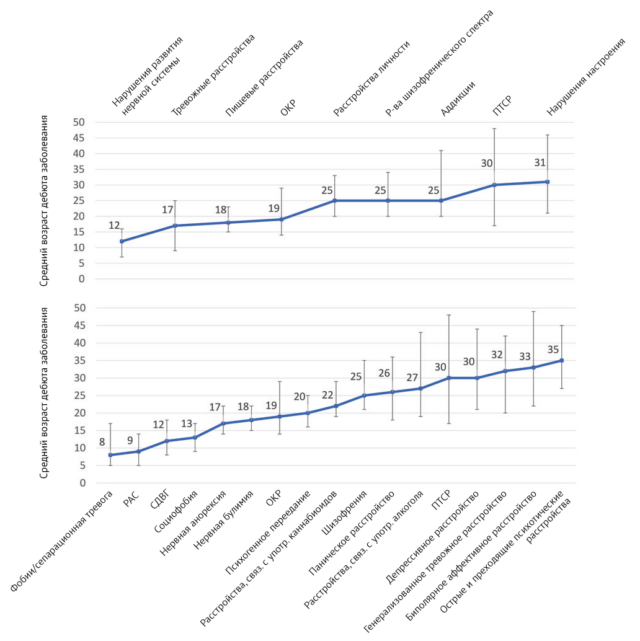
\includegraphics[width=0.8\linewidth]{figures/Students_issue.png}
  \caption{A statistics about students age and their issues.}
\end{figure}

\vspace{0.5cm}
\justifying
 Today, most students face a lack of opportunities and fear in communication, as well as to ask for help for mutually beneficial exchange of skills and also experience and support for their educational projects and ideas within the universities themselves. Despite the different online platforms on the internet and the initiatives of educational institutions, you say that universities have many clubs for the development of new abilities, for example: a music club or a programming club, yes, it helps but not everyone, perhaps the university gives a direction to help the student community, but it is not always not everyone uses it because of fear in communication. 
\par
\vspace{0.5cm}
Many of them have difficulties and fears in finding suitable resources and platforms and are also limited in communicating with students to get the necessary help to implement their ideas and projects or mutually beneficial exchange.  
\newpage
Limited access (not in all universities) to high-quality educational materials, some materials may be outdated, restrictions on social contact, some students are afraid to make contact, which may affect in the future and lack of financial support for their ideas, implementation, influence, and so on, hinders the process of skill development, which may hinder the expansion of students' knowledge bases and the formation of professional relations within the university environment. 
\par
\vspace{0.5cm}
Such problems can affect the motivation of students, the realization of learning, personal development, and prospects for professional growth of students, which potentially affects both academic success and future careers.
Let's give some student fears, student fears are provocateurs of mental disorders in students.
As you can see in the picture above "\nameref{fig:sstats}", the main part of the students are young people \textbf{aged 17-25 years.} During this age period, the risk of many mental disorders increases. 
In 2021, the journal Molecular Psychiatry \cite{student-fears} published the results of a meta-analysis of 192 epidemiological studies from around the world, according to which the following psychopathologies are highly likely to debut at this age.

\par
\vspace{0.5cm}
\textbf{Eating disorders} - anorexia nervosa, bulimia nervosa, psychogenic overeating \cite{student-fears}.

\par
\vspace{0.5cm}
\textbf{Obsessive} compulsive disorders — are the appearance of obsessive, disturbing, or frightening thoughts (obsessions) and obsessive actions (compulsions) \cite{student-fears}.

\par
\vspace{0.5cm}
\textbf{Personality disorders}  —  are a distorted perception of reality and inadequate ways of responding to events \cite{student-fears}.

\par
\vspace{0.5cm}
\textbf{Schizophrenic disorders} — are fundamental disorders of thinking and perception that can be accompanied by auditory hallucinations, false memories, fantastic delusions, and social dysfunction \cite{student-fears}.

\par
\vspace{0.5cm}
\textbf{Addiction} — is the desire to escape reality and change your mental state with the help of psychotropic substances \cite{student-fears}.

\vspace{0.5cm}
Also, according to our survey, "\nameref{survqa6}" conducted in 2024 this semester, it turned out that when asked do you have a lot of friends at the university, it turned out that \textbf{53.8} percent have very few friends at universities, that is, they have few connections to live life in the future, that is, theoretically it will not be much harder to live who did not live who has more connections, therefore our application partially solves this problem.

\newpage
\section{Thesis Outline}\label{thesis}
\hspace*{0.5cm} The first chapter of our document is an "\nameref{ch:intro}" in which we describe our goals and motivation and describe the existing problem related to this project. The second chapter contains, "\nameref{ch:A}" information that will help readers understand how a mutually beneficial skills exchange project is carried out and not only help our country specifically for students in comparing other cases from different countries. In the third chapter, we describe the "\nameref{ch:B}" we used during the development of our project and how we distributed the responsibilities. In the fourth chapter, we describe about "\nameref{ch:C}" we do analyze competitive and product analysis by the topic our project. In the fifth chapter, we describe the "\nameref{ch:D}" of which stack technologies how we used starting our project from prototyping and ending MVP product and in the last section we describe the "\nameref{ch:E}" of the project and its further development.
